% ============================================================
%  DCN Finals Reviewer
%  Polytechnic University of the Philippines
%  Data Communication and Networking | June 2026
% ============================================================
\documentclass[9pt]{article}

% -- Fonts ---------------------------------------------------
% SFNS is the installed macOS system typeface: SF Pro.
\usepackage{fontspec}
\setmainfont{SFNS.ttf}[
  Path=/System/Library/Fonts/,
  UprightFont=SFNS.ttf,
  BoldFont=SFNS.ttf,
  ItalicFont=SFNSItalic.ttf,
  BoldItalicFont=SFNSItalic.ttf,
  BoldFeatures={FakeBold=2},
  BoldItalicFeatures={FakeBold=2}
]

% -- Page geometry (8.5 x 13 in — Philippine Long / Foolscap)
\usepackage[
  paperwidth=8.5in,
  paperheight=13in,
  top=0.55in,
  bottom=0.55in,
  left=0.45in,
  right=0.45in,
  headheight=18.65pt,
  headsep=0.12in,
  footskip=0.3in
]{geometry}

% -- Colour --------------------------------------------------
\usepackage{xcolor}
\definecolor{themeColor}{HTML}{660100}
\definecolor{InkBlack}{HTML}{1A1A1A}
\definecolor{MutedGray}{HTML}{66615B}
\definecolor{SurfaceWhite}{HTML}{FFFFFF}
\definecolor{AnswerRed}{HTML}{8B1A1A}
\definecolor{LightRedBg}{HTML}{FDF2F2}
\definecolor{LightBlueBg}{HTML}{EEF4FB}
\definecolor{SoftBlue}{HTML}{4A7FB5}
\color{InkBlack}

% -- Layout --------------------------------------------------
\usepackage{multicol}
\setlength{\columnsep}{0.28in}
\setlength{\columnseprule}{0.4pt}
\def\columnseprulecolor{\color{themeColor!30}}

% -- Section Headings ----------------------------------------
\usepackage{titlesec}
\titleformat{\section}
  {\large\bfseries\color{themeColor}}{\thesection.}{0.5em}{}[\vspace{-0.4em}\rule{\linewidth}{0.5pt}]
\titleformat{\subsection}
  {\normalsize\bfseries\color{themeColor}}{\thesubsection.}{0.5em}{}
\titlespacing*{\section}{0pt}{0.7em}{0.2em}
\titlespacing*{\subsection}{0pt}{0.5em}{0.15em}

% -- Lists ---------------------------------------------------
\usepackage{enumitem}
\setlist{nosep, leftmargin=1.2em}
\usepackage{tabularx}

% -- Boxes ---------------------------------------------------
\usepackage[most]{tcolorbox}

% -- Links ---------------------------------------------------
\usepackage[colorlinks=true, linkcolor=themeColor, urlcolor=themeColor]{hyperref}

% -- Header / Footer -----------------------------------------
\usepackage{fancyhdr}
\pagestyle{fancy}
\fancyhf{}
\lhead{\footnotesize\color{themeColor}\bfseries DCN Finals Reviewer}
\rhead{\footnotesize\color{MutedGray} Data Communication \& Networking}
\cfoot{\small\color{MutedGray}\thepage}
\renewcommand{\headrulewidth}{0.4pt}
\renewcommand{\headrule}{\hbox to\headwidth{\color{themeColor}\leaders\hrule height \headrulewidth\hfill}}

% -- Misc ----------------------------------------------------
\usepackage{microtype}
\usepackage{ragged2e}
\usepackage{tikz}
\usetikzlibrary{arrows.meta,positioning}
\usepackage{eso-pic}
\usepackage{needspace}
\raggedbottom
\raggedcolumns
\setlength{\parindent}{0pt}
\setlength{\parskip}{0pt}

\tikzset{
  mindroot/.style={
    draw=themeColor,
    fill=themeColor!10,
    rounded corners=5pt,
    thick,
    text width=2.1cm,
    align=center,
    font=\scriptsize\bfseries,
    inner sep=5pt
  },
  mindleaf/.style={
    draw=SoftBlue!60,
    fill=LightBlueBg,
    rounded corners=4pt,
    text width=2.55cm,
    align=left,
    font=\scriptsize,
    inner sep=4pt
  },
  mindaccent/.style={
    draw=themeColor!45,
    fill=LightRedBg,
    rounded corners=4pt,
    text width=2.55cm,
    align=left,
    font=\scriptsize,
    inner sep=4pt
  },
  mindline/.style={
    draw=themeColor!55,
    -{Latex[length=1.8mm]},
    line width=0.45pt
  }
}



% ============================================================
%  CUSTOM COMMANDS
% ============================================================

% Full-width answer tag so long answers wrap cleanly.
\newcommand{\answer}[1]{%
  \par\nobreak\vspace{1pt}%
  \begin{tcolorbox}[
    colback=AnswerRed,
    colframe=AnswerRed,
    boxrule=0pt,
    arc=0pt,
    left=4pt, right=4pt,
    top=0.5pt, bottom=0.5pt,
    before skip=0pt,
    after skip=0pt
  ]
  {\footnotesize\bfseries\color{white}\RaggedRight #1}
  \end{tcolorbox}
}

% Highlighted important word/phrase — bold + theme colour
\newcommand{\hl}[1]{\textbf{\textcolor{themeColor}{#1}}}

% Explanation box — subtle red-tinted background
\newcommand{\explain}[1]{%
  \par\nobreak\vspace{0pt}%
  \begin{tcolorbox}[
    colback=LightBlueBg,
    colframe=SoftBlue!30,
    boxrule=0.3pt,
    arc=2pt,
    left=4pt, right=4pt,
    top=1pt, bottom=1pt,
    before skip=1pt,
    after skip=2pt
  ]
  {\footnotesize\color{MutedGray}\RaggedRight\itshape #1}
  \end{tcolorbox}
}

% Question item
\newcounter{qnum}
\newcommand{\question}[1]{%
  \Needspace{4\baselineskip}%
  \stepcounter{qnum}%
  \par\vspace{3pt}%
  {\footnotesize\bfseries\color{themeColor}\theqnum.}\ {\footnotesize #1}%
}

\newcommand{\memorybox}[2]{%
  \begin{tcolorbox}[
    colback=LightRedBg,
    colframe=themeColor!35,
    boxrule=0.4pt,
    arc=2pt,
    left=5pt, right=5pt,
    top=4pt, bottom=4pt,
    before skip=3pt,
    after skip=4pt
  ]
  {\bfseries\color{themeColor}#1}\par\vspace{2pt}
  {\small\RaggedRight #2}
  \end{tcolorbox}
}

\newcommand{\scopepage}[2]{%
  \begin{tcolorbox}[
    colback=LightBlueBg,
    colframe=SoftBlue!35,
    boxrule=0.45pt,
    arc=3pt,
    left=7pt, right=7pt,
    top=6pt, bottom=6pt,
    before skip=4pt,
    after skip=5pt
  ]
  {\bfseries\color{themeColor}LaTeX mind map}\par\vspace{3pt}
  {\small\RaggedRight #1}
  \end{tcolorbox}
  \begin{tcolorbox}[
    colback=LightRedBg,
    colframe=themeColor!35,
    boxrule=0.45pt,
    arc=3pt,
    left=7pt, right=7pt,
    top=6pt, bottom=6pt,
    before skip=4pt,
    after skip=6pt
  ]
  {\bfseries\color{themeColor}Cheat sheet / quick visual}\par\vspace{3pt}
  {\small\RaggedRight #2}
  \end{tcolorbox}
}

\newcommand{\questioncolumns}[1]{%
  \begin{multicols}{2}
  \subsection*{Practice Questions}
  #1
  \end{multicols}
}

% ============================================================
\begin{document}
\thispagestyle{fancy}

% -- Title Block ---------------------------------------------
\begin{center}
  {\LARGE\bfseries\color{themeColor} DCN Finals Reviewer\par}
  \vspace{0.08cm}
  {\normalsize\itshape Data Communication and Networking\par}
  \vspace{0.04cm}
  {\color{themeColor}\rule{0.5\textwidth}{1pt}}
\end{center}
\vspace{0.04cm}

\begin{multicols}{2}

% ============================================================
\section*{How to Use This Reviewer}
% ============================================================

\memorybox{Exam-scope order}{
This reviewer is now grouped by the six exam scopes: \textbf{Network Layer}, \textbf{IPv4 Concepts}, \textbf{IPv6 Concepts}, \textbf{Transport Layer}, \textbf{Application Layer}, and \textbf{Network Security Fundamentals}. Each scope starts with a LaTeX-drawn mind map and a quick visual before the questions.
}

% ============================================================
\section*{Acronyms to Memorize First}
% ============================================================

\memorybox{High-yield full names}{
\begin{itemize}[leftmargin=1em]
  \item \textbf{DHCP} --- Dynamic Host Configuration Protocol
  \item \textbf{DNS} --- Domain Name System
  \item \textbf{FTP/TFTP} --- File Transfer Protocol / Trivial File Transfer Protocol
  \item \textbf{HTTP/HTTPS} --- Hypertext Transfer Protocol / Secure
  \item \textbf{SMTP, POP, IMAP} --- Email send and retrieval protocols
  \item \textbf{SMB} --- Server Message Block
  \item \textbf{URL} --- Uniform Resource Locator
  \item \textbf{IP, IPv4, IPv6} --- Internet Protocol versions
  \item \textbf{GUA, LLA, ULA} --- Global, Link-Local, and Unique Local IPv6 addresses
  \item \textbf{RA/RS} --- Router Advertisement / Router Solicitation
  \item \textbf{TCP/UDP} --- Transmission Control Protocol / User Datagram Protocol
  \item \textbf{MSS, MTU, SACK, ISN} --- Segment size, link size, selective ACK, initial sequence number
  \item \textbf{AAA} --- Authentication, Authorization, Accounting
  \item \textbf{DMZ} --- Demilitarized Zone
  \item \textbf{SPI} --- Stateful Packet Inspection
  \item \textbf{IANA} --- Internet Assigned Numbers Authority
\end{itemize}
}

% ============================================================
\section*{Most Likely to Ask}
% ============================================================

\memorybox{Focus pass before answering drills}{
\begin{itemize}[leftmargin=1em]
  \item \textbf{Network layer}: logical addressing, encapsulation, routing, fragmentation, best effort, connectionless delivery.
  \item \textbf{IPv4}: network/host portions, subnet mask, ANDing, private ranges, broadcast, loopback, NAT, VLSM.
  \item \textbf{IPv6}: 128-bit hex addresses, hextets, compression, GUA/LLA/ULA, ff02::1 and ff02::2 multicast, RA/RS, Hop Limit.
  \item \textbf{Transport}: TCP reliable/ordered/stateful; UDP connectionless/low overhead; ports identify application conversations.
  \item \textbf{Application}: HTTP methods, URL parts, DNS records, DHCP DORA, email protocols, FTP ports, P2P/client-server models.
  \item \textbf{Security}: threats, vulnerabilities, malware, attack types, firewall filtering, AAA, DMZ, password/SSH hardening.
\end{itemize}
}

\end{multicols}

\clearpage
\section{Network Layer}
\scopepage{
\begin{center}
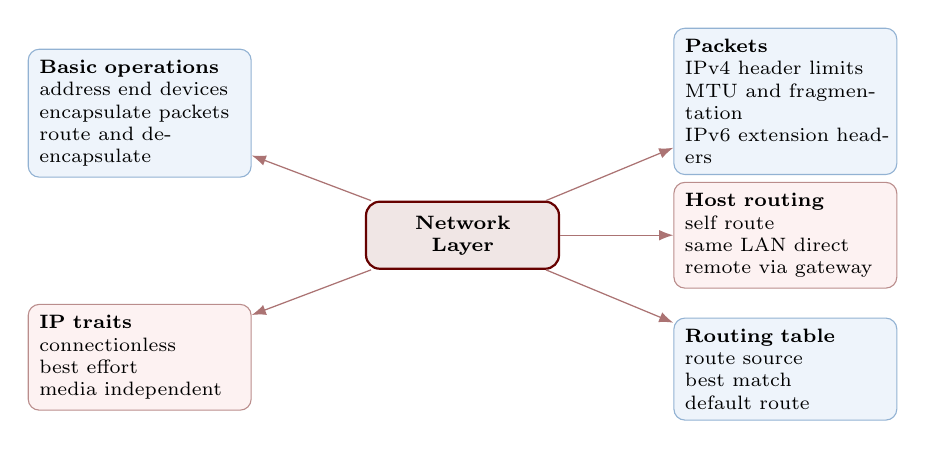
\begin{tikzpicture}[x=1cm,y=1cm]
  \node[mindroot] (root) at (0,0) {Network\\Layer};
  \node[mindleaf] (ops) at (-4.1,1.55) {\textbf{Basic operations}\\address end devices\\encapsulate packets\\route and de-encapsulate};
  \node[mindaccent] (ip) at (-4.1,-1.55) {\textbf{IP traits}\\connectionless\\best effort\\media independent};
  \node[mindleaf] (packet) at (4.1,1.7) {\textbf{Packets}\\IPv4 header limits\\MTU and fragmentation\\IPv6 extension headers};
  \node[mindaccent] (host) at (4.1,0) {\textbf{Host routing}\\self route\\same LAN direct\\remote via gateway};
  \node[mindleaf] (table) at (4.1,-1.7) {\textbf{Routing table}\\route source\\best match\\default route};
  \foreach \target in {ops,ip,packet,host,table}{\draw[mindline] (root) -- (\target);}
\end{tikzpicture}
\end{center}
}{
\begin{center}
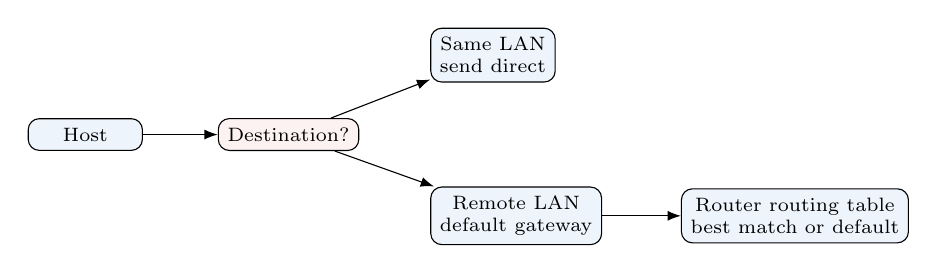
\begin{tikzpicture}[>=Latex, node distance=0.95cm, every node/.style={font=\scriptsize, align=center}]
  \node[draw, rounded corners, fill=LightBlueBg, minimum width=1.45cm] (host) {Host};
  \node[draw, rounded corners, fill=LightRedBg, right=of host] (decision) {Destination?};
  \node[draw, rounded corners, fill=LightBlueBg, above right=0.45cm and 0.9cm of decision] (local) {Same LAN\\send direct};
  \node[draw, rounded corners, fill=LightBlueBg, below right=0.45cm and 0.9cm of decision] (remote) {Remote LAN\\default gateway};
  \node[draw, rounded corners, fill=LightBlueBg, right=1.0cm of remote] (router) {Router routing table\\best match or default};
  \draw[->] (host) -- (decision);
  \draw[->] (decision) -- (local);
  \draw[->] (decision) -- (remote);
  \draw[->] (remote) -- (router);
\end{tikzpicture}
\end{center}
\begin{itemize}[leftmargin=1em]
  \item \textbf{IP packet =} Network Layer PDU.
  \item \textbf{IPv4 fragmentation} happens when a packet is too large for the link MTU; IPv6 routers do not fragment packets.
  \item \textbf{Route source} tells how a router learned the route: connected, static, EIGRP, and so on.
\end{itemize}
}

\questioncolumns{
\question{Which routes are automatically added by a router when an interface is active and has addressing?}

\answer{Directly Connected}

\explain{A directly connected route appears automatically for networks attached to active, addressed router interfaces.}


\question{Which route forwards traffic in a specific direction when there is no matching entry in the routing table?}

\answer{Default Route}

\explain{A default route is the fallback path used when a packet's destination does not match a more specific route.}


\question{What does it mean for IP to be \hl{connectionless}?}

\answer{IP does not establish a connection with the destination before sending the packet}

\explain{Connectionless delivery means each packet is sent independently without first creating an end-to-end session.}


\question{Which type of route must be manually configured and adjusted by a network administrator?}

\answer{Static Route}

\explain{Static routes are entered by an administrator and do not automatically change when network conditions change.}


\question{What occurs when Layer 3 splits an IPv4 packet into smaller units?}

\answer{Fragmentation}

\explain{Fragmentation divides a packet into smaller pieces so it can fit across a link with a smaller maximum transmission unit.}


\question{Which code in a Cisco routing table indicates an EIGRP learned route?}

\answer{D}

\explain{Cisco routing tables use the code D for routes learned through EIGRP.}


\question{True or False: IP is considered unreliable because it cannot manage or fix undelivered or corrupt packets.}

\answer{True}

\explain{IP provides no built-in recovery for lost, delayed, duplicate, or corrupt packets; reliability is handled by upper-layer protocols when needed.}


\question{What represents the \hl{Network Layer PDU}?}

\answer{IP Packet}

\explain{At the network layer, the protocol data unit is a packet, commonly an IP packet.}


\question{Which characteristic says IP does not guarantee delivery of a packet?}

\answer{Best Effort}

\explain{Best effort means IP attempts delivery but does not guarantee arrival, order, or error recovery.}


\question{In a router's routing table, what does the Route Source entry identify?}

\answer{How the network was learned by the router}

\explain{The route source code, such as C for connected or D for EIGRP, tells how the router learned the route.}


\question{What is the primary function of Read-only memory (ROM) in a Cisco router?}

\answer{To provide startup instructions and perform the Power-on self-test (POST)}

\explain{ROM contains essential boot microcode and hardware self-test instructions.}
}

\clearpage
\section{IPv4 Concepts}
\scopepage{
\begin{center}
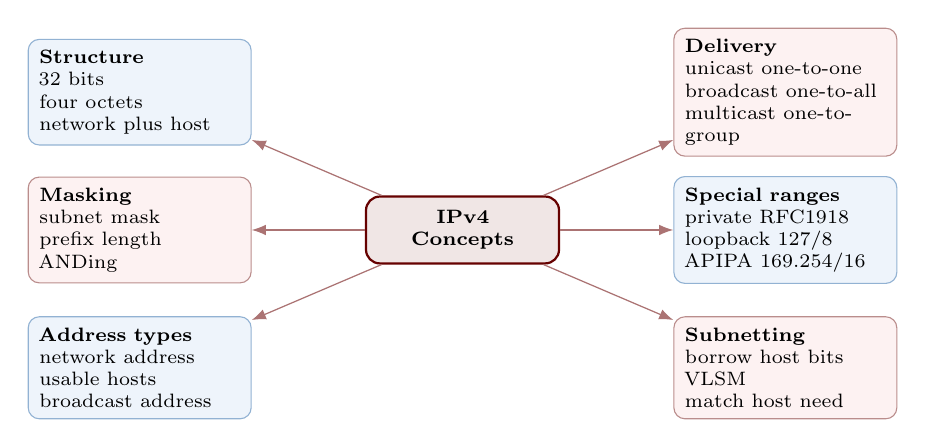
\begin{tikzpicture}[x=1cm,y=1cm]
  \node[mindroot] (root) at (0,0) {IPv4\\Concepts};
  \node[mindleaf] (structure) at (-4.1,1.75) {\textbf{Structure}\\32 bits\\four octets\\network plus host};
  \node[mindaccent] (mask) at (-4.1,0) {\textbf{Masking}\\subnet mask\\prefix length\\ANDing};
  \node[mindleaf] (types) at (-4.1,-1.75) {\textbf{Address types}\\network address\\usable hosts\\broadcast address};
  \node[mindaccent] (comm) at (4.1,1.75) {\textbf{Delivery}\\unicast one-to-one\\broadcast one-to-all\\multicast one-to-group};
  \node[mindleaf] (special) at (4.1,0) {\textbf{Special ranges}\\private RFC1918\\loopback 127/8\\APIPA 169.254/16};
  \node[mindaccent] (subnet) at (4.1,-1.75) {\textbf{Subnetting}\\borrow host bits\\VLSM\\match host need};
  \foreach \target in {structure,mask,types,comm,special,subnet}{\draw[mindline] (root) -- (\target);}
\end{tikzpicture}
\end{center}
}{
\begin{tabularx}{\linewidth}{@{}>{\bfseries}l X@{}}
Example & \texttt{192.168.10.15/24} \\
Network bits & first 24 bits = \texttt{192.168.10} \\
Host bits & last 8 bits = \texttt{15} \\
Network address & \texttt{192.168.10.0} \\
Broadcast & \texttt{192.168.10.255} \\
\end{tabularx}
\vspace{4pt}
\begin{center}
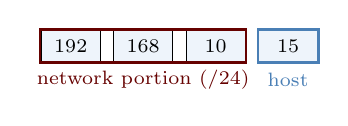
\begin{tikzpicture}[x=0.92cm,y=0.5cm,every node/.style={font=\scriptsize}]
  \foreach \x/\label in {0/192,1/168,2/10,3/15}{\node[draw, minimum width=.75cm, minimum height=.45cm, fill=LightBlueBg] at (\x,0) {\label};}
  \draw[themeColor, thick] (-.42,-.42) rectangle (2.42,.42);
  \draw[SoftBlue, thick] (2.58,-.42) rectangle (3.42,.42);
  \node[themeColor] at (1,-.85) {network portion (/24)};
  \node[SoftBlue] at (3,-.85) {host};
\end{tikzpicture}
\end{center}
\textbf{Borrowing formula:} borrowed bits \(n\) create \(2^n\) subnets.
}

\questioncolumns{
\question{How many total bits make up a standard \hl{IPv4 address} structure?}

\answer{32}

\explain{An IPv4 address is a 32-bit number, typically written as four decimal octets separated by dots (e.g., 192.168.1.1).}


\question{Which component is used by a network device to differentiate the \hl{network portion} from the \hl{host portion} of an IPv4 address?}

\answer{Subnet Mask}

\explain{The subnet mask is a 32-bit value where contiguous 1-bits mark the network portion and 0-bits mark the host portion of an address.}


\question{What is the logical result of the \hl{ANDing process} when a binary 1 is compared to a binary 0?}

\answer{0}

\explain{The AND operation returns 1 only when both bits are 1; any other combination (1\,\&\,0, 0\,\&\,1, 0\,\&\,0) yields 0.}


\question{What is the \hl{prefix length} for a subnet mask of \hl{255.255.255.0}?}

\answer{/24}

\explain{Three octets of all 1s (8 $\times$ 3) equals 24 bits set in the mask.}


\question{According to \hl{RFC 1918}, which of the following is a \hl{private IPv4 address} range?}

\answer{192.168.0.0/16}

\explain{This range is reserved for internal network use and is not globally routable.}


\question{What is sending a packet to all other destination IP addresses called?}

\answer{Broadcast}

\explain{Broadcast communication sends one packet to every host on the destination network.}


\question{What translates private IPv4 addresses to public IPv4 addresses?}

\answer{Network Address Translation (NAT)}

\explain{NAT lets private internal addresses communicate externally by translating them to public IPv4 addresses.}


\question{What are addresses commonly known as Automatic Private IP Addressing (APIPA) or self-assigned addresses?}

\answer{Link-Local Address}

\explain{IPv4 link-local/APIPA addresses are self-assigned when a host cannot obtain an address from DHCP.}


\question{Which address category is commonly identified by \texttt{127.0.0.1}?}

\answer{Loopback Addresses}

\explain{Loopback addresses let a host send traffic to itself for testing and local services.}


\question{What is the bit value in the \hl{Version} field for an IPv4 packet?}

\answer{0100}

\explain{IPv4 is version 4, represented in the 4-bit Version field as 0100.}


\question{What two portions make up an IPv4 address?}

\answer{Network and host}

\explain{The network portion identifies the network, while the host portion identifies the specific device on that network.}


\question{Which process determines the network address from an IPv4 address and subnet mask?}

\answer{ANDing}

\explain{The IPv4 address and subnet mask are compared bit by bit; the result is the network address.}


\question{If you borrow 1 bit from the host portion of a /24 network, how many subnets are created?}

\answer{2}

\explain{Borrowing \(n\) bits creates \(2^n\) subnets; \(2^1\) equals 2.}


\question{What is the benefit of using Variable Length Subnet Masking (VLSM)?}

\answer{It allows subnets of different sizes and reduces unused host addresses}

\explain{VLSM lets each subnet match the needed host count instead of forcing every subnet to be the same size.}


\question{A host with IP address \texttt{192.168.10.15/24} belongs to which network address?}

\answer{192.168.10.0}

\explain{With a /24 mask, the final octet is the host portion; setting it to 0 gives the network address.}


\question{What is the broadcast address for the network \texttt{172.16.0.0/16}?}

\answer{172.16.255.255}

\explain{A /16 leaves the final two octets for hosts; setting all host bits to 1 gives 255.255.}


\question{How many bits are borrowed to create 8 subnets?}

\answer{3 bits}

\explain{\(2^3\) creates 8 subnets.}


\question{If an administrator needs to create 30 subnets, how many bits must be borrowed from a /24 network?}

\answer{5 bits}

\explain{Borrowing 5 bits creates 32 subnets, the smallest power of 2 that can cover 30.}


\question{Which statement describes a slash /24 octet boundary?}

\answer{The network portion ends after the third octet}

\explain{Each octet is 8 bits, so 24 bits means the first three octets are the network portion.}


\question{What is the result of borrowing 2 bits from the third octet of a /8 network?}

\answer{A /10 prefix}

\explain{Adding 2 borrowed bits to the original /8 prefix produces /10.}


\question{A company uses \texttt{10.0.0.0/8} and needs subnets for 200 hosts each. Which prefix length is most appropriate?}

\answer{/24}

\explain{A /24 subnet provides 254 usable host addresses, enough for 200 hosts with less waste than a larger subnet.}


\question{If you have a /16 network and need to create 256 subnets, what will be the new prefix length?}

\answer{/24}

\explain{Creating 256 subnets requires borrowing 8 bits; 16 + 8 = 24.}


\question{What is the theoretical maximum number of addresses provided by IPv4?}

\answer{4.3 billion}

\explain{IPv4 uses 32 bits, giving \(2^{32}\) possible addresses, or about 4.3 billion.}
}

\clearpage
\section{IPv6 Concepts}
\scopepage{
\begin{center}
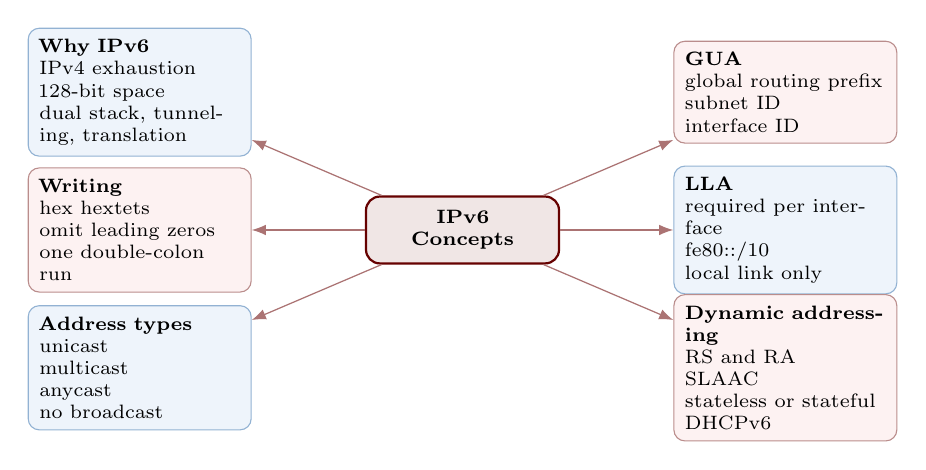
\begin{tikzpicture}[x=1cm,y=1cm]
  \node[mindroot] (root) at (0,0) {IPv6\\Concepts};
  \node[mindleaf] (why) at (-4.1,1.75) {\textbf{Why IPv6}\\IPv4 exhaustion\\128-bit space\\dual stack, tunneling, translation};
  \node[mindaccent] (write) at (-4.1,0) {\textbf{Writing}\\hex hextets\\omit leading zeros\\one double-colon run};
  \node[mindleaf] (types) at (-4.1,-1.75) {\textbf{Address types}\\unicast\\multicast\\anycast\\no broadcast};
  \node[mindaccent] (gua) at (4.1,1.75) {\textbf{GUA}\\global routing prefix\\subnet ID\\interface ID};
  \node[mindleaf] (lla) at (4.1,0) {\textbf{LLA}\\required per interface\\fe80::/10\\local link only};
  \node[mindaccent] (dynamic) at (4.1,-1.75) {\textbf{Dynamic addressing}\\RS and RA\\SLAAC\\stateless or stateful DHCPv6};
  \foreach \target in {why,write,types,gua,lla,dynamic}{\draw[mindline] (root) -- (\target);}
\end{tikzpicture}
\end{center}
}{
\begin{tabularx}{\linewidth}{@{}>{\bfseries}l X@{}}
\texttt{ff02::1} & All-nodes multicast group: all IPv6 interfaces on the local link listen. \\
\texttt{ff02::2} & All-routers multicast group: IPv6 routers listen after routing is enabled. \\
\texttt{fe80::/10} & Link-local address range; stays on the local link. \\
\texttt{2000::/3} & Currently assigned Global Unicast Address range. \\
\end{tabularx}
\vspace{4pt}
\begin{center}
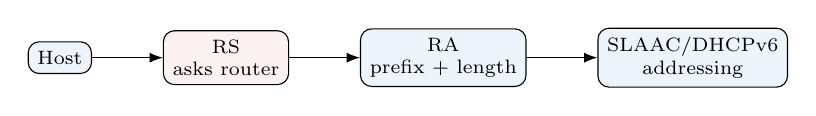
\begin{tikzpicture}[>=Latex, node distance=.9cm, every node/.style={font=\scriptsize, align=center}]
  \node[draw, rounded corners, fill=LightBlueBg] (host) {Host};
  \node[draw, rounded corners, fill=LightRedBg, right=of host] (rs) {RS\\asks router};
  \node[draw, rounded corners, fill=LightBlueBg, right=of rs] (ra) {RA\\prefix + length};
  \node[draw, rounded corners, fill=LightBlueBg, right=of ra] (addr) {SLAAC/DHCPv6\\addressing};
  \draw[->] (host) -- (rs); \draw[->] (rs) -- (ra); \draw[->] (ra) -- (addr);
\end{tikzpicture}
\end{center}
}

\questioncolumns{
\question{The devices run both \hl{IPv4} and \hl{IPv6} protocol stacks simultaneously.}

\answer{Dual Stack}

\explain{Dual stack allows a single device to process both IPv4 and IPv6 packets independently on the same interface.}


\question{A method of transporting an \hl{IPv6 packet} over an \hl{IPv4 network}. The IPv6 packet is \hl{encapsulated} inside an IPv4 packet.}

\answer{Tunneling}

\explain{Tunneling wraps (encapsulates) an IPv6 packet inside an IPv4 header so it can traverse IPv4-only infrastructure without modification.}


\question{Which IPv6 transition mechanism lets IPv6-only devices communicate with IPv4-only devices by \hl{converting packet headers} between the two protocols?}

\answer{Translation}

\explain{Translation converts packet headers between IPv6 and IPv4 formats, enabling direct communication between hosts running different IP versions.}


\question{Uniquely identifies an \hl{interface} on an IPv6-enabled device.}

\answer{Unicast}

\explain{A unicast address identifies exactly one interface; packets sent to a unicast address are delivered to that single destination.}


\question{Used to send a single IPv6 packet to \hl{multiple destinations}.}

\answer{Multicast}

\explain{Multicast delivers a packet to all members of a specific group, reducing bandwidth usage compared to sending individual copies to each recipient.}


\question{Any IPv6 unicast address that can be assigned to \hl{multiple devices}. A packet sent to this address is routed to the \hl{nearest device} having that address.}

\answer{Anycast}

\explain{Anycast uses routing metrics to forward the packet to the topologically closest interface sharing the same address, improving latency and redundancy.}


\question{Similar to a \hl{public IPv4 address}. These are \hl{globally unique, internet-routable} addresses.}

\answer{Global Unicast Address (GUA)}

\explain{GUAs are assigned from the 2000::/3 range and are equivalent to public IPv4 addresses, allowing devices to be reached across the global Internet.}


\question{Which IPv6 address type is required on every enabled interface, supports communication on the same \hl{local link}, and is \hl{not routable} beyond that link?}

\answer{Link-Local Address (LLA)}

\explain{Link-local addresses (fe80::/10) are automatically configured on every IPv6 interface and are used for neighbor discovery and routing protocol exchanges within a single network segment.}


\question{A \hl{multicast group} that \hl{all IPv6-enabled devices} join. A packet sent to this group is received and processed by all IPv6 interfaces on the link or network.}

\answer{ff02::1 All-Nodes Multicast Group}

\explain{ff02::1 is the link-local scope all-nodes multicast address, analogous to a broadcast in IPv4—every IPv6 host on the link listens to this address.}


\question{A \hl{multicast group} that \hl{all IPv6 routers} join. A router becomes a member of this group when it is enabled as an IPv6 router with the \texttt{ipv6 unicast-routing} global configuration command.}

\answer{ff02::2 All-Routers Multicast Group}

\explain{ff02::2 targets only routers on the local link; hosts send Router Solicitation messages to this address to discover available routers.}


\question{What is the total address length of an IPv6 address and written in what format?}

\answer{128, Hexadecimal}

\explain{IPv6 utilizes a 128-bit address space to provide a significantly larger number of unique addresses compared to IPv4.}


\question{The unofficial term used to refer to a segment of \hl{16 bits}, or \hl{four hexadecimal values}.}

\answer{Hextet}

\explain{A hextet refers to a four-hexadecimal digit segment representing 16 bits of the 128-bit address.}


\question{According to \hl{Rule 1} of IPv6 compression, which zeros can be omitted?}

\answer{Leading Zeros in Any Hextet}

\explain{Only zeros at the start of a hextet can be omitted without making the address ambiguous.}


\question{Which of the following is a valid compression of the address \texttt{2001:0db8:0000:1111:0000:0000:0000:0200}?}

\answer{2001:db8:0:1111::200}

\explain{This correctly applies Rule 1 (leading zeros) and Rule 2 (double colon for a contiguous string of all-zero hextets).}


\question{True or False: IPv6 addresses are \hl{case-sensitive}.}

\answer{False}

\explain{IPv6 addresses are not case-sensitive and can be written in lowercase, uppercase, or a mix of both.}


\question{Which address type did IPv6 \hl{eliminate} that was present in IPv4?}

\answer{Broadcast}

\explain{IPv6 does not have a broadcast address, using specific multicast groups instead to reduce unnecessary network noise.}


\question{What is the recommended \hl{prefix length} for most IPv6 LANs?}

\answer{/64}

\explain{A 64-bit interface ID is required for SLAAC and simplifies network management and subnetting.}


\question{\hl{Global Unicast Addresses (GUAs)} currently being assigned always begin with which \hl{binary bits}?}

\answer{001}

\explain{The binary prefix `001' corresponds to the 2000::/3 address space currently used for GUAs.}


\question{Which field in a Global Unicast Address lies between the provider-assigned network portion and the host-identifying portion, allowing an organization to \hl{identify internal subnets}?}

\answer{Subnet ID}

\explain{This field allows organizations to create internal subnets within their allocated global routing prefix.}


\question{Which field in a Global Unicast Address is the \hl{network portion assigned by a provider}, such as an ISP, to a customer or site?}

\answer{Global Routing Prefix}

\explain{This portion forms the network identity that is routable on the global Internet.}


\question{Which field in an IPv6 address is equivalent to the \hl{host portion} of an IPv4 address and is normally \hl{64 bits long} on a /64 subnet?}

\answer{Interface ID}

\explain{The Interface ID uniquely identifies a host on a specific subnet.}


\question{What is the specific address range for \hl{IPv6 Link-Local Addresses (LLAs)}?}

\answer{fe80::/10}

\explain{LLAs are required for every interface and always fall within the fe80::/10 range.}


\question{What prefix range is used by \hl{Unique Local Addresses (ULAs)}?}

\answer{fc00::/7 to fdff::/7}

\explain{ULAs are used for local addressing within a site and fall within this specific range.}


\question{In the \hl{EUI-64 process}, what value is inserted into the \hl{middle of the 48-bit MAC address}?}

\answer{fffe}

\explain{The EUI-64 process takes the 48-bit MAC and inserts the 16-bit hex value `fffe' in the middle to create a 64-bit ID.}


\question{Which \hl{ICMPv6 message} is sent by a router to provide \hl{addressing information} to hosts?}

\answer{Router Advertisement (RA)}

\explain{Routers send RA messages periodically or in response to an RS to provide prefix and gateway data.}


\question{How often do IPv6 routers typically send out \hl{unsolicited ICMPv6 RA messages}?}

\answer{Every 200 seconds}

\explain{By default, IPv6-enabled routers send RA messages every 200 seconds to all nodes.}


\question{What is the restriction when applying IPv6 compression \hl{Rule 2}, the double colon?}

\answer{It can only be used once within an address}

\explain{The double colon replaces one contiguous sequence of all-zero hextets; using it more than once would make the original address ambiguous.}


\question{What is the decimal equivalent of the address space provided by IPv6?}

\answer{340 undecillion addresses}

\explain{IPv6 provides $2^{128}$ possible addresses, approximately 340 undecillion unique addresses.}


\question{Where are IPv6 Extension Headers (EH) placed in a packet?}

\answer{Between the IPv6 header and the payload}

\explain{Extension headers follow the main IPv6 header and appear before the transport-layer payload.}


\question{Which IPv6 header field indicates the size of the data portion of the packet?}

\answer{Payload Length}

\explain{Payload Length specifies the size of the data following the main IPv6 header.}


\question{Which organization developed IPv6?}

\answer{Internet Engineering Task Force (IETF)}

\explain{IPv6 was developed by the IETF to address IPv4 exhaustion and modernize IP addressing.}


\question{What is the binary representation of the \hl{Version} field in an IPv6 header?}

\answer{0110}

\explain{IPv6 is version 6, represented in the 4-bit Version field as 0110.}


\question{In what hex range do all currently assigned IPv6 Global Unicast Addresses (GUAs) fall?}

\answer{2000::/3}

\explain{Currently assigned GUAs begin with binary 001, which corresponds to addresses in 2000::/3.}


\question{If an IPv6-enabled interface is not manually configured with an LLA, what will the device do?}

\answer{It will automatically create one}

\explain{IPv6 requires a link-local address on enabled interfaces, so devices can generate one automatically.}


\question{Which ICMPv6 message is sent by a host to discover IPv6 routers on the network?}

\answer{Router Solicitation (RS)}

\explain{A host sends an RS message to ask routers to provide configuration information immediately.}


\question{What does a Router Advertisement (RA) message typically provide to a host?}

\answer{Network prefix and prefix length}

\explain{RA messages provide the prefix information a host can use for SLAAC or related IPv6 configuration.}


\question{Which IPv6 header field is the equivalent of the IPv4 Time-to-Live (TTL) field?}

\answer{Hop Limit}

\explain{Hop Limit is decremented at each hop to prevent packets from looping forever.}


\question{How does the size of an IPv6 header compare to a standard IPv4 header?}

\answer{The IPv6 header is larger, 40 bytes versus 20 bytes}

\explain{IPv6 has a simplified fixed header, but its 128-bit addresses make the base header 40 bytes.}
}

\clearpage
\section{Transport Layer}
\scopepage{
\begin{center}
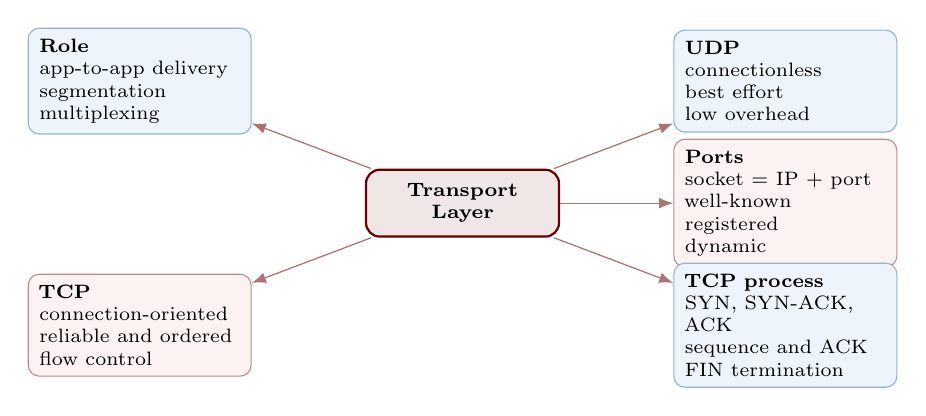
\begin{tikzpicture}[x=1cm,y=1cm]
  \node[mindroot] (root) at (0,0) {Transport\\Layer};
  \node[mindleaf] (role) at (-4.1,1.55) {\textbf{Role}\\app-to-app delivery\\segmentation\\multiplexing};
  \node[mindaccent] (tcp) at (-4.1,-1.55) {\textbf{TCP}\\connection-oriented\\reliable and ordered\\flow control};
  \node[mindleaf] (udp) at (4.1,1.55) {\textbf{UDP}\\connectionless\\best effort\\low overhead};
  \node[mindaccent] (ports) at (4.1,0) {\textbf{Ports}\\socket = IP + port\\well-known\\registered\\dynamic};
  \node[mindleaf] (process) at (4.1,-1.55) {\textbf{TCP process}\\SYN, SYN-ACK, ACK\\sequence and ACK\\FIN termination};
  \foreach \target in {role,tcp,udp,ports,process}{\draw[mindline] (root) -- (\target);}
\end{tikzpicture}
\end{center}
}{
\begin{center}
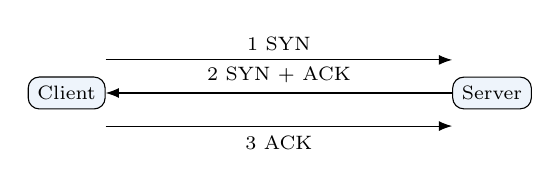
\begin{tikzpicture}[>=Latex, node distance=0.8cm, every node/.style={font=\scriptsize, align=center}]
  \node[draw, rounded corners, fill=LightBlueBg] (client) {Client};
  \node[draw, rounded corners, fill=LightBlueBg, right=4.4cm of client] (server) {Server};
  \draw[->] ([yshift=.42cm]client.east) -- node[above] {1 SYN} ([yshift=.42cm]server.west);
  \draw[<-] (client.east) -- node[above] {2 SYN + ACK} (server.west);
  \draw[->] ([yshift=-.42cm]client.east) -- node[below] {3 ACK} ([yshift=-.42cm]server.west);
\end{tikzpicture}
\end{center}
\begin{tabularx}{\linewidth}{@{}>{\bfseries}l X@{}}
TCP & reliable, ordered, flow control, retransmission, higher overhead \\
UDP & low delay, low overhead, no built-in retransmission \\
Ports & 0--1023 well-known; 1024--49151 registered; 49152--65535 dynamic \\
\end{tabularx}
}

\questioncolumns{
\question{Responsible for establishing a temporary communication session between two applications and delivering data between them.}

\answer{Transport Layer}

\explain{The transport layer manages end-to-end communication by establishing sessions and ensuring data reaches the correct application.}


\question{Which transport layer protocol is considered 'reliable' because it supports packet delivery confirmation?}

\answer{TCP}

\explain{TCP uses sequence numbers and acknowledgments to ensure all data is delivered and processed.}


\question{What is the overhead size of a standard TCP header?}

\answer{20 bytes}

\explain{The TCP header contains several fields for reliability and flow control, totaling 20 bytes of overhead.}


\question{Which TCP flag is used to abruptly terminate a session if necessary?}

\answer{RST}

\explain{The Reset (RST) flag is used to immediately close a connection without the standard handshake.}


\question{Which is a 'Stateless' protocol?}

\answer{UDP}

\explain{UDP does not track session data or confirm delivery, making it stateless.}


\question{When using \texttt{netstat -n}, what does the '-n' option do?}

\answer{Displays IP addresses and port numbers in numerical form.}

\explain{This prevents the utility from attempting to resolve addresses to names, speeding up the output.}


\question{In a TCP session termination, which flag is used by the client to indicate it has no more data to send?}

\answer{FIN}

\explain{The Finish (FIN) flag signals the end of data transmission from that side of the connection.}


\question{What is the primary role of the 'Destination Port' in a header?}

\answer{To identify the service or application running on the server.}

\explain{Ports like 80 or 443 tell the receiving OS which software should handle the incoming data.}


\question{Which layer is responsible for \hl{logical communications between applications} running on different hosts?}

\answer{Transport Layer}

\explain{The transport layer provides end-to-end logical communication between application processes on different devices.}


\question{Which layer is the \hl{link between the application layer and the lower layers} responsible for network transmission?}

\answer{Transport Layer}

\explain{The transport layer accepts application data, segments it, and passes it to the lower layers for network delivery.}


\question{Which characteristic is a hallmark of the \hl{User Datagram Protocol (UDP)}?}

\answer{Connectionless Best-Effort Delivery}

\explain{UDP does not establish a formal session before sending data and does not provide acknowledgments for received packets.}


\question{Which TCP flag indicates that the \hl{urgent pointer field} is significant?}

\answer{URG}

\explain{The URG flag tells the receiver that the urgent pointer field should be interpreted as urgent data information.}


\question{Which TCP flag is the \hl{acknowledgment flag} used in connection establishment and session termination?}

\answer{ACK}

\explain{The ACK flag confirms that data or control information has been received and identifies the next expected byte.}


\question{Which TCP flag represents the \hl{push function}?}

\answer{PSH}

\explain{The PSH flag asks the receiver to pass buffered data to the application as soon as possible.}


\question{Which TCP flag \hl{resets the connection} when an error or timeout occurs?}

\answer{RST}

\explain{The RST flag abruptly terminates a TCP connection when the session cannot continue normally.}


\question{Which TCP flag \hl{synchronizes sequence numbers} during connection establishment?}

\answer{SYN}

\explain{The SYN flag starts a TCP session by synchronizing initial sequence numbers between endpoints.}


\question{Which TCP flag means \hl{no more data from the sender} and is used in session termination?}

\answer{FIN}

\explain{The FIN flag tells the other endpoint that the sender has finished transmitting data.}


\question{What is the \hl{maximum amount of data} that the destination device can receive in a TCP segment called?}

\answer{Maximum Segment Size (MSS)}

\explain{MSS defines the largest TCP payload that can be sent in one segment without including the IP and TCP headers.}


\question{If an IPv4 packet has an Ethernet \hl{MTU of 1500 bytes}, what is the typical TCP Maximum Segment Size for data?}

\answer{1460 bytes}

\explain{Subtracting the 20-byte IPv4 header and the 20-byte TCP header from the 1500-byte MTU leaves 1460 bytes for TCP data.}


\question{What is the purpose of \hl{Selective Acknowledgment (SACK)} in TCP?}

\answer{To explicitly acknowledge which segments were received}

\explain{SACK lets the receiver identify received and missing byte ranges, so the sender retransmits only the missing pieces.}


\question{True or False: UDP is considered a \hl{stateful protocol} because it monitors the status of the connection.}

\answer{False}

\explain{UDP is stateless; it sends data without tracking a session or checking whether the destination is ready to receive.}


\question{During TCP session termination, how many steps are typically involved to close the connection in both directions?}

\answer{Four}

\explain{TCP termination normally uses a FIN and ACK from one side, followed by a FIN and ACK from the other side.}


\question{Which TCP header field is a \hl{16-bit field} used to identify the source application by port number?}

\answer{Source Port}

\explain{The source port identifies the sending application or process on the source host.}


\question{Which TCP header field is a \hl{16-bit field} used to identify the destination application by port number?}

\answer{Destination Port}

\explain{The destination port identifies the service or application that should receive the segment.}


\question{Which TCP header field is a \hl{32-bit field} used for data reassembly purposes?}

\answer{Sequence Number}

\explain{The sequence number identifies the order of bytes so TCP can reassemble data correctly.}


\question{Which TCP header field is a \hl{32-bit field} used to indicate that data has been received and to identify the next byte expected?}

\answer{Acknowledgment Number}

\explain{The acknowledgment number confirms receipt and tells the sender which byte the receiver expects next.}


\question{Which TCP header field is a \hl{4-bit field} also known as the data offset?}

\answer{Header Length}

\explain{Header Length indicates the size of the TCP segment header so the receiver can locate the data payload.}


\question{Which TCP header field is a \hl{6-bit field} reserved for future use?}

\answer{Reserved}

\explain{The reserved field is kept for future TCP extensions and should normally be set to zero.}


\question{Which TCP header field contains bit codes or flags that indicate the \hl{purpose and function} of the TCP segment?}

\answer{Control Bits}

\explain{Control bits include flags such as URG, ACK, PSH, RST, SYN, and FIN.}


\question{Which TCP header field is a \hl{16-bit field} that indicates how many bytes can be accepted at one time?}

\answer{Window Size}

\explain{Window Size supports flow control by advertising how much data the receiver can accept.}


\question{Which TCP header field is a \hl{16-bit field} used for error checking of the segment header and data?}

\answer{Checksum}

\explain{The checksum helps detect corruption in the TCP header and data.}


\question{Which TCP header field is a \hl{16-bit field} used to indicate if the contained data is urgent?}

\answer{Urgent Pointer}

\explain{The urgent pointer is meaningful when the URG flag is set and points to urgent data in the segment.}


\question{What is the combination of an \hl{IP address and port number} known as?}

\answer{Socket}

\explain{A socket identifies an endpoint by combining an IP address with a transport-layer port number.}


\question{Which protocol is best suited for applications that tolerate some data loss but cannot tolerate delays, such as live audio streaming?}

\answer{UDP}

\explain{UDP avoids retransmission and connection overhead, making it useful for time-sensitive traffic where speed matters more than perfect delivery.}


\question{What congestion behavior results in packets being \hl{discarded by an overloaded router}?}

\answer{Congestion Avoidance}

\explain{When congestion avoidance mechanisms detect overload, excess packets may be dropped to protect the network from collapse.}


\question{What endpoint identifier is used to identify the \hl{server and service} being requested by a client?}

\answer{Socket}

\explain{The destination socket combines the server IP address and destination port for the requested service.}


\question{What is the IANA range for \hl{well-known ports}?}

\answer{0 to 1023}

\explain{Ports 0 through 1023 are reserved for common services such as HTTP, FTP, DNS, and SSH.}


\question{Which network utility can verify \hl{active connections} in a host?}

\answer{netstat}

\explain{\texttt{netstat} displays active network connections, routing tables, and interface statistics.}


\question{Which port number is typically associated with \hl{HTTP}?}

\answer{80}

\explain{Port 80 is the well-known port for standard unencrypted HTTP web traffic.}


\question{What is the \hl{Initial Sequence Number (ISN)} in a TCP connection?}

\answer{A randomly chosen sequence number used during TCP session setup}

\explain{The ISN is chosen during connection setup and then incremented by the number of transmitted bytes.}


\question{True or False: A single server can host both a web service on port 80 and an FTP service on port 21 at the same time.}

\answer{True}

\explain{A server can run multiple services simultaneously because each service listens on a different port number.}


\question{Which standards body assigns addressing standards, including port numbers?}

\answer{Internet Assigned Numbers Authority (IANA)}

\explain{IANA manages global coordination of DNS root data, IP addressing, and protocol resources such as port numbers.}


\question{Which flag is used in the first step of the TCP session termination process?}

\answer{FIN}

\explain{The FIN flag begins graceful session termination by indicating that the sender has no more data to transmit.}


\question{Which protocol is a better choice for an application that requires all data to be fully received before any of it is useful, such as a software update?}

\answer{TCP}

\explain{TCP provides reliability, ordering, acknowledgments, and retransmission, which are required for complete file delivery.}


\question{TCP and UDP both use which layer of the TCP/IP model?}

\answer{Transport}

\explain{TCP and UDP are transport-layer protocols that manage end-to-end delivery between applications.}


\question{What port number range is used for Registered Ports as assigned by IANA?}

\answer{1,024 to 49,151}

\explain{Registered ports are assigned to requesting entities for specific applications and services.}


\question{Which well-known port is used for the control connection of FTP sessions?}

\answer{21}

\explain{FTP uses port 21 for control commands and port 20 for data transfer in active FTP.}


\question{How many bits are used for the Source Port and Destination Port fields in both TCP and UDP headers?}

\answer{16 bits each}

\explain{Both TCP and UDP use 16-bit source and destination port fields, allowing port numbers from 0 to 65,535.}


\question{Which feature is unique to TCP compared to UDP?}

\answer{Flow control}

\explain{TCP uses flow control to prevent the sender from overwhelming the receiver; UDP does not.}


\question{What is the total size of a standard UDP header?}

\answer{8 bytes}

\explain{The UDP header has four 16-bit fields: source port, destination port, length, and checksum.}


\question{Which application layer protocol uses UDP port 69 and requires reliability to be handled by the application itself?}

\answer{TFTP}

\explain{Trivial File Transfer Protocol uses UDP port 69, so the application must handle reliability behavior.}


\question{Which protocol is connection-oriented and supports same-order delivery?}

\answer{TCP}

\explain{TCP establishes a session and uses sequence numbers so data can be delivered reliably and in order.}


\question{What is the primary advantage of using UDP for live video and multimedia applications?}

\answer{It provides minimal delay by not retransmitting lost data or waiting for acknowledgments}

\explain{Real-time media usually values low latency more than perfect retransmission.}


\question{Which port number is used by the Simple Mail Transfer Protocol (SMTP)?}

\answer{25}

\explain{SMTP commonly uses well-known port 25 for mail transfer.}


\question{What happens during Step 2 of the TCP three-way handshake?}

\answer{The server responds with SYN and ACK flags}

\explain{The server acknowledges the client SYN and sends its own SYN to synchronize sequence numbers.}


\question{What port range is typically used by a client's operating system as ephemeral ports?}

\answer{49,152 to 65,535}

\explain{Private or dynamic ports identify temporary client-side conversations.}


\question{Which port number is used by the DHCP server to listen for requests?}

\answer{67}

\explain{DHCP servers listen on UDP port 67, while clients use UDP port 68.}
}

\clearpage
\section{Application Layer}
\scopepage{
\begin{center}
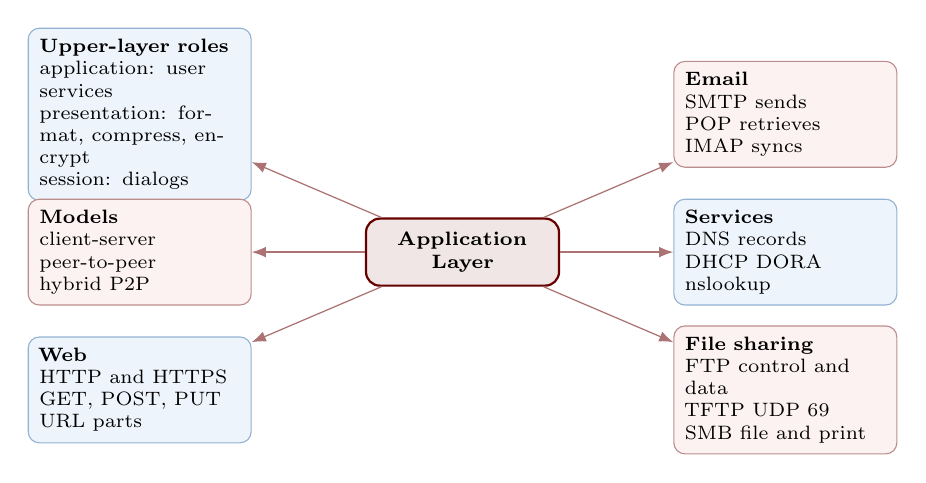
\begin{tikzpicture}[x=1cm,y=1cm]
  \node[mindroot] (root) at (0,0) {Application\\Layer};
  \node[mindleaf] (layers) at (-4.1,1.75) {\textbf{Upper-layer roles}\\application: user services\\presentation: format, compress, encrypt\\session: dialogs};
  \node[mindaccent] (models) at (-4.1,0) {\textbf{Models}\\client-server\\peer-to-peer\\hybrid P2P};
  \node[mindleaf] (web) at (-4.1,-1.75) {\textbf{Web}\\HTTP and HTTPS\\GET, POST, PUT\\URL parts};
  \node[mindaccent] (email) at (4.1,1.75) {\textbf{Email}\\SMTP sends\\POP retrieves\\IMAP syncs};
  \node[mindleaf] (services) at (4.1,0) {\textbf{Services}\\DNS records\\DHCP DORA\\nslookup};
  \node[mindaccent] (file) at (4.1,-1.75) {\textbf{File sharing}\\FTP control and data\\TFTP UDP 69\\SMB file and print};
  \foreach \target in {layers,models,web,email,services,file}{\draw[mindline] (root) -- (\target);}
\end{tikzpicture}
\end{center}
}{
\begin{center}
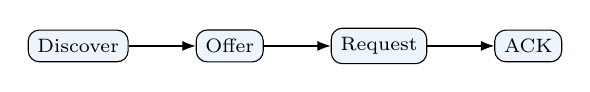
\begin{tikzpicture}[>=Latex, node distance=.85cm, every node/.style={font=\scriptsize, align=center}]
  \node[draw, rounded corners, fill=LightBlueBg] (discover) {Discover};
  \node[draw, rounded corners, fill=LightBlueBg, right=of discover] (offer) {Offer};
  \node[draw, rounded corners, fill=LightBlueBg, right=of offer] (request) {Request};
  \node[draw, rounded corners, fill=LightBlueBg, right=of request] (ack) {ACK};
  \draw[->] (discover) -- (offer); \draw[->] (offer) -- (request); \draw[->] (request) -- (ack);
\end{tikzpicture}
\end{center}
\begin{tabularx}{\linewidth}{@{}>{\bfseries}l X@{}}
URL & \texttt{http://www.cisco.com/index.html} = protocol + server name + filename \\
SMTP & sends mail, port 25 \\
POP & downloads/retrieves, commonly removes from server \\
IMAP & synchronizes mail while originals remain on server \\
DNS records & A = IPv4, AAAA = IPv6, NS = name server, MX = mail exchange \\
FTP & pull = download; control port 21, data port 20 \\
\end{tabularx}
}

\questioncolumns{
\question{The layer that is closest to the \hl{end user}.}

\answer{Application Layer}

\explain{The Application layer is the topmost layer of both the OSI and TCP/IP models, providing the interface through which users interact with network services such as HTTP, FTP, and DNS.}


\question{A client/server file sharing protocol.}

\answer{Server Message Block (SMB)}


\question{What are the 3 primary functions of the presentation layer?}

\answer{Format data, Compress data, Encrypt data}


\question{Another protocol used to retrieve email messages.}

\answer{IMAP}


\question{Allows the user to manually place DNS queries.}

\answer{nslookup}


\question{Which protocol is a 'request/response' protocol that specifies GET, POST, and PUT message types and is not secure. Messages can be intercepted.}

\answer{HTTP}

\explain{The Hypertext Transfer Protocol uses these specific request methods to interact with resources on a web server.}


\question{When a DHCP lease must be renewed, which message does the client send?}

\answer{DHCPREQUEST}

\explain{A client sends a REQUEST message to ask for an extension of its existing lease before it expires.}


\question{Which message type is sent by a DHCP server if an IP address offer is no longer valid?}

\answer{DHCPNAK}

\explain{A negative acknowledgment (NAK) tells the client that the server cannot fulfill the specific request.}


\question{Which layer of the OSI model is responsible for providing the \hl{interface between user applications and the network}?}

\answer{Application Layer}

\explain{The Application layer is closest to the end user and serves as the primary interface for network-aware applications.}


\question{Which layer of the OSI model is responsible for creating and maintaining \hl{dialogs} between source and destination applications?}

\answer{Session Layer}

\explain{The Session layer manages the exchange of information to keep conversations active and restart them if necessary.}


\question{What is the primary role of a \hl{tracker} in BitTorrent technology?}

\answer{To keep track of which files are hosted by which users}

\explain{Trackers maintain records of which peers have specific file segments so other peers can locate and share them.}


\question{Which layer of the OSI model formats data at the source device into a format compatible with the destination device?}

\answer{Presentation Layer}

\explain{The Presentation layer helps ensure that data sent from the Application layer of one system can be read by the Application layer of another.}


\question{Which DNS resource record type maps a domain name to an \hl{IPv6 address}?}

\answer{AAAA}

\explain{The quad-A record is designed for 128-bit IPv6 addresses.}


\question{Which DHCP message is broadcast by a client to find available servers when it first connects to a network?}

\answer{DHCPDISCOVER}

\explain{The client uses DHCPDISCOVER to locate DHCP servers on the local network segment.}


\question{Which HTTP method is a client request for data, such as when a web browser requests an HTML page?}

\answer{GET}

\explain{GET asks the web server to return a requested resource.}


\question{Which HTTP method uploads data files or form data to a web server?}

\answer{POST}

\explain{POST sends data to a server for processing, such as submitted form contents.}


\question{Which HTTP method uploads or replaces resources or content on a web server, such as an image?}

\answer{PUT}

\explain{PUT sends a resource to the server, commonly to create or replace content at a specified location.}


\question{Which graphic image format mentioned in the material is a common standard handled at the Presentation layer?}

\answer{PNG}

\explain{Portable Network Graphics (PNG) is a common image format handled as presentation-layer data formatting.}


\question{What is a distinguishing characteristic of a Peer-to-Peer (P2P) network model?}

\answer{Every connected device can act as both a client and a server}

\explain{P2P roles are decentralized; a peer can request a resource in one transaction and provide one in another.}


\question{How does a hybrid P2P system differ from a standard P2P system?}

\answer{An index server helps peers locate resources while resource sharing remains decentralized}

\explain{Hybrid P2P keeps peer-to-peer file sharing but uses a central index or tracker to help peers find who has the resource.}


\question{What are the three basic parts of a URL such as protocol, server name, and filename?}

\answer{Protocol, server name, and specific filename}

\explain{A URL identifies the scheme or protocol, the host or server name, and the resource or file being requested.}


\question{What is the primary difference between HTTP and HTTPS?}

\answer{HTTPS uses authentication and encryption to secure data}

\explain{HTTP sends data without encryption; HTTPS protects the session so intercepted traffic cannot be read easily.}


\question{A store-and-forward method of sending, storing, and retrieving electronic messages.}

\answer{Email}

\explain{Email stores messages on servers until the recipient retrieves or synchronizes them.}


\question{What is a major advantage of using IMAP over POP for retrieving email?}

\answer{It lets users view copies of messages while the originals remain on the server}

\explain{IMAP keeps mail on the server and synchronizes state, which is useful when the same mailbox is opened from many devices.}


\question{Which DNS record type is used to identify an authoritative name server?}

\answer{NS}

\explain{An NS record names the authoritative DNS servers for a zone.}


\question{In the DNS hierarchy, which top-level domain represents a non-profit organization?}

\answer{.org}

\explain{The .org top-level domain is commonly associated with non-profit organizations.}


\question{What happens to a DHCP-distributed IP address when it is no longer in use?}

\answer{It is returned to the address pool for reuse}

\explain{DHCP leases allow unused addresses to return to the pool so another host can receive them later.}


\question{Which protocol is primarily used for file-sharing and print services in Windows-based networking?}

\answer{Server Message Block (SMB)}

\explain{SMB is the common Windows resource-sharing protocol for files, printers, and related services.}


\question{What is the function of the DNS MX record?}

\answer{A mail exchange record identifies where email for a domain should be delivered}

\explain{MX records point sending mail servers to the mail exchangers responsible for a domain.}


\question{What Windows command displays all cached DNS entries?}

\answer{\texttt{ipconfig /displaydns}}

\explain{The /displaydns option shows the local DNS resolver cache.}


\question{What is the function of the DNS A record?}

\answer{It maps a name to an end-device IPv4 address}

\explain{An A record links a human-readable host name to a 32-bit IPv4 address.}


\question{Which common video file standard is processed at the Presentation layer?}

\answer{MPEG}

\explain{MPEG is a common video standard, so it fits the presentation-layer role of formatting data.}


\question{What port number does an SMTP client typically use to connect to a mail server?}

\answer{25}

\explain{SMTP uses well-known port 25 to transfer email between mail systems.}


\question{How does an FTP client pull data from a server?}

\answer{By downloading a file}

\explain{Pulling data means the client requests and receives a file from the server.}


\question{In the DNS hierarchy, what do top-level domains like .au or .co usually represent?}

\answer{Country-code top-level domains}

\explain{Two-letter TLDs are usually country-code top-level domains assigned to countries or territories.}


\question{True or False: Application layer protocols must be implemented in both the source and destination devices to allow communication.}

\answer{True}

\explain{Both endpoints must use compatible protocol rules to understand the same application-layer exchange.}
}

\clearpage
\section{Network Security Fundamentals}
\scopepage{
\begin{center}
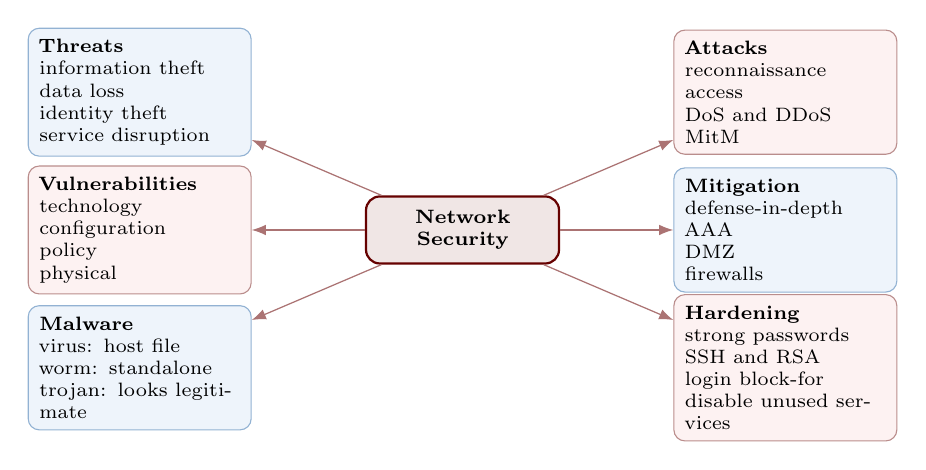
\begin{tikzpicture}[x=1cm,y=1cm]
  \node[mindroot] (root) at (0,0) {Network\\Security};
  \node[mindleaf] (threats) at (-4.1,1.75) {\textbf{Threats}\\information theft\\data loss\\identity theft\\service disruption};
  \node[mindaccent] (vulns) at (-4.1,0) {\textbf{Vulnerabilities}\\technology\\configuration\\policy\\physical};
  \node[mindleaf] (malware) at (-4.1,-1.75) {\textbf{Malware}\\virus: host file\\worm: standalone\\trojan: looks legitimate};
  \node[mindaccent] (attacks) at (4.1,1.75) {\textbf{Attacks}\\reconnaissance\\access\\DoS and DDoS\\MitM};
  \node[mindleaf] (mitigation) at (4.1,0) {\textbf{Mitigation}\\defense-in-depth\\AAA\\DMZ\\firewalls};
  \node[mindaccent] (hardening) at (4.1,-1.75) {\textbf{Hardening}\\strong passwords\\SSH and RSA\\login block-for\\disable unused services};
  \foreach \target in {threats,vulns,malware,attacks,mitigation,hardening}{\draw[mindline] (root) -- (\target);}
\end{tikzpicture}
\end{center}
}{
\begin{tabularx}{\linewidth}{@{}>{\bfseries}l X@{}}
Authentication & Who are you? \\
Authorization & What are you allowed to do? \\
Accounting & What did you do? \\
Packet filtering & IP/MAC allow or block rules \\
Application filtering & allows or blocks by port/application type \\
URL filtering & allows or blocks by URLs or keywords \\
SPI & permits legitimate replies, blocks unsolicited packets \\
DMZ & controlled public-service subnet separated from the inside network \\
\end{tabularx}
}

\questioncolumns{
\question{The \hl{discovery and mapping} of systems, services, or vulnerabilities.}

\answer{Reconnaissance Attacks}

\explain{Reconnaissance is the information-gathering phase where attackers probe networks using tools like ping sweeps and port scans to identify potential targets.}


\question{The unauthorized \hl{manipulation of data}, system access, or \hl{user privileges}.}

\answer{Access Attacks}

\explain{Access attacks exploit authentication weaknesses or software vulnerabilities to gain unauthorized entry to systems or escalate privileges.}


\question{The \hl{disabling or corruption} of networks, systems, or services.}

\answer{Denial of Service}

\explain{DoS attacks flood a target with traffic or exploit protocol weaknesses to exhaust resources, rendering the service unavailable to legitimate users.}


\question{A type of malware that propagates by \hl{inserting a copy of itself} into, and becoming part of, another program. It spreads from one computer to another, leaving infections as it travels.}

\answer{Viruses}

\explain{Viruses require a host file to propagate; they attach to legitimate programs and execute when the host program runs.}


\question{Similar to viruses in that they \hl{replicate functional copies} of themselves and can cause the same type of damage. In contrast to viruses, which require the spreading of an infected host file, this is a \hl{standalone software} and does not require a \hl{host program} or human help to propagate.}

\answer{Worms}

\explain{Worms are self-propagating and exploit network vulnerabilities to spread automatically without user interaction or a host executable.}


\question{A harmful piece of software that \hl{looks legitimate}. They do not reproduce by infecting other files. They \hl{self-replicate} and spread through \hl{user interaction} such as opening an email attachment or downloading and running a file from the internet.}

\answer{Trojan Horses}

\explain{Trojans disguise themselves as useful software to trick users into installing them, after which they can create backdoors, steal data, or download additional malware.}


\question{Malware is short for\ldots}

\answer{Malicious Software}

\explain{``Malware'' is the umbrella term for any software intentionally designed to cause damage, including viruses, worms, trojans, ransomware, and spyware.}


\question{Includes \hl{physical damage} to servers, routers, switches, cabling plant, and workstations.}

\answer{Hardware Threats}

\explain{Hardware threats encompass any event—accidental or deliberate—that physically damages networking equipment, such as vandalism, theft, or natural disasters.}


\question{Includes \hl{temperature extremes} (too hot or too cold) or \hl{humidity extremes} (too wet or too dry).}

\answer{Environmental Threats}

\explain{Environmental threats affect equipment reliability; excessive heat causes overheating, while high humidity can lead to condensation and corrosion on circuit boards.}


\question{Includes \hl{voltage spikes}, insufficient supply voltage (\hl{brownouts}), unconditioned power (\hl{noise}), and \hl{total power loss}.}

\answer{Electrical Threats}

\explain{Electrical threats are mitigated by using UPS (uninterruptible power supplies), surge protectors, and power conditioners to maintain clean, stable electricity.}


\question{Includes \hl{poor handling} of key electrical components (\hl{electrostatic discharge}), lack of critical spare parts, poor cabling, and poor labeling.}

\answer{Maintenance Threats}

\explain{Maintenance threats arise from neglecting best practices such as ESD wrist straps, proper cable management, and keeping an adequate inventory of spare parts.}


\question{Implemented using \hl{brute force}, \hl{Trojan horse}, and \hl{packet sniffers}.}

\answer{Password Attacks}

\explain{Password attacks attempt to discover credentials through exhaustive guessing (brute force), keystroke logging (Trojans), or intercepting unencrypted credentials on the network (sniffers).}


\question{A threat actor uses \hl{unauthorized privileges} to gain access to a system, possibly compromising the target.}

\answer{Trust Exploitation}

\explain{Trust exploitation abuses the trust relationships between systems—e.g., if System A trusts System B, compromising B gives the attacker access to A.}


\question{A threat actor uses a \hl{compromised system} as a base for attacks against other targets. For example, using \hl{SSH (port 22)} to connect to a compromised host A. Host A is trusted by host B and, therefore, the threat actor can use \hl{Telnet (port 23)} to access it.}

\answer{Port Redirection}

\explain{Port redirection (pivoting) allows an attacker to tunnel traffic through a compromised host to reach otherwise inaccessible systems on the internal network.}


\question{The threat actor is positioned \hl{in between two legitimate entities} in order to \hl{read or modify} the data that passes between the two parties.}

\answer{Man-in-the-Middle}

\explain{MitM attacks intercept communications in real time, enabling eavesdropping, session hijacking, or data manipulation without either party's knowledge.}


\question{Prevents or allows access based on \hl{IP or MAC addresses}.}

\answer{Packet Filtering}

\explain{Packet filtering examines the source and destination addresses in each packet header and applies allow/deny rules without inspecting payload content.}


\question{Prevents or allows access by specific \hl{application types} based on \hl{port numbers}.}

\answer{Application Filtering}

\explain{Application filtering controls traffic by matching well-known port numbers (e.g., port 80 for HTTP, port 443 for HTTPS) to allow or block specific services.}


\question{Prevents or allows access to websites based on specific \hl{URLs or keywords}.}

\answer{URL Filtering}

\explain{URL filtering inspects the requested web address or embedded keywords and blocks access to sites that match a deny list or policy category.}


\question{Which firewall filtering method tracks active connections, permits incoming packets that are \hl{legitimate responses} to internal requests, and blocks \hl{unsolicited packets} unless explicitly allowed?}

\answer{Stateful Packet Inspection (SPI)}

\explain{SPI maintains a state table of active connections and only permits inbound traffic that corresponds to an established outbound session, providing stronger security than simple packet filtering.}


\question{Which term describes intruders who gain access by modifying software or exploiting software vulnerabilities?}

\answer{Threat actors}

\explain{Threat actors are individuals or groups that exploit weaknesses to gain unauthorized access or cause harm.}


\question{A network suffers from a weakness in the TCP/IP protocol itself. Which vulnerability category is this?}

\answer{Technological vulnerabilities}

\explain{Protocol, operating system, and hardware weaknesses are technological vulnerabilities.}


\question{Which item is considered a configuration vulnerability?}

\answer{Unsecured user accounts}

\explain{Weak or default account settings are configuration problems.}


\question{Which malware is a standalone program that replicates itself and does not need a host program to spread?}

\answer{Worm}

\explain{A worm is independent software that can replicate across networks without attaching to a host file.}


\question{Which tool might a threat actor use during reconnaissance to determine the IP address space assigned to a corporation?}

\answer{nslookup}

\explain{Tools such as nslookup and whois help gather DNS, domain, and address information.}


\question{What is the term for infected hosts controlled by a command-and-control program to perform attacks?}

\answer{Botnet}

\explain{A botnet is a group of compromised hosts controlled together for attacks such as DDoS.}


\question{Which security approach combines networking devices and services in a layered fashion?}

\answer{Defense-in-depth}

\explain{Defense-in-depth layers controls so another protection can help when one control fails.}


\question{Which part of AAA determines exactly what a user is allowed to do while logged into the network?}

\answer{Authorization}

\explain{Authorization defines permitted actions and resources after identity is verified.}


\question{Which AAA component keeps a record of what the user did while accessing the network?}

\answer{Accounting}

\explain{Accounting logs user activity for audits, tracking, and accountability.}


\question{Where are servers accessible to outside users usually placed to allow controlled access without compromising the internal network?}

\answer{Demilitarized Zone (DMZ)}

\explain{A DMZ exposes public services in a controlled subnet while separating them from the internal network.}


\question{Why is securing endpoint devices one of the most challenging jobs for a network administrator?}

\answer{It involves human nature and user behavior}

\explain{Endpoint security depends on technical controls and on users following safe practices.}


\question{What is the minimum recommended length for a strong password?}

\answer{Eight characters}

\explain{Eight characters is a common minimum, while longer passwords or passphrases are stronger.}


\question{What is a passphrase in Cisco device security?}

\answer{A phrase made of many words that is longer and harder to guess}

\explain{A passphrase uses multiple words to create something long, memorable, and more resistant to guessing.}


\question{Which Cisco command prevents plaintext passwords from being visible in the configuration file?}

\answer{\texttt{service password-encryption}}

\explain{This command encrypts plaintext passwords in the running configuration.}


\question{What is the purpose of the command \texttt{login block-for 120 attempts 3 within 60}?}

\answer{To deter brute-force password guessing attacks}

\explain{The command blocks login attempts after repeated failures within a short period.}


\question{What is the minimum recommended RSA key modulus length for secure SSH configuration?}

\answer{1024 bits}

\explain{Cisco guidance commonly treats 1024 bits as the minimum practical RSA key size for SSH.}


\question{In Cisco IOS-XE, which command verifies which ports are currently open on the device?}

\answer{\texttt{show ip ports all}}

\explain{This command displays open IP ports on IOS-XE devices.}
}
\vspace{0.5em}
\begin{center}
  {\color{themeColor}\rule{0.6\linewidth}{0.8pt}}\\[4pt]
  {\footnotesize\itshape\color{MutedGray} End of Reviewer}
\end{center}

\end{document}
